\chaptertoc{}

\section{Matériel et méthodes}

	\subsection{Modèle animal}

	\lipsum[1]\index{Lorem ipsum}

	Une première note de fin de document\endnote{Première note de fin de document.}, une deuxième\endnote{Deuxième note de fin de document.} et \ldots \endnote{\ldots note de fin de document.} \endnote{\ldots note de fin de document.} \endnote{\ldots note de fin de document.} \endnote{\ldots note de fin de document.} \endnote{\ldots note de fin de document.} \endnote{\ldots note de fin de document.} \endnote{\ldots note de fin de document.}: le package enotez associé à hyperref permet l'appel et le retour de note\endnote{\lipsum[1]\index{Lorem ipsum}}.

	\subsection{Traitement expérimental}

		\subsubsection{Hypergravité}
			\label{hypergravite} % on peut mettre systématiquement un \label après chaque titre de partie au cas où un appel \ref{} serait nécessaire

			L'hypergravité consiste à augmenter la force du vecteur gravitaire en lui sur-imposant la force centrifuge. En effet, la force centrifuge induite par la rotation se surimpose à la gravité terrestre ce qui permet d'avoir une force résultante dépendante de la vitesse de rotation. On utilise pour cela des centrifugeuses qui sont des carrousels équipés de nacelles suspendues à des axes libres permettant à la force résultante d'être perpendiculaire au plancher de la nacelle et ainsi obtenir une «gravité» dont la force est supérieure à la gravité terrestre tout en maintenant, pour les individus expérimentaux, l'orientation \og naturelle \fg de celle-ci.
		
		\subsubsection{La centrifugeuse}

			Les caractéristiques techniques de la centrifugeuse\index{centrifugeuse} ont été décrites dans un article de~\cite{jamon_ground-based_2008} et dans la partie~\ref{hypergravite}. Brièvement, la centrifugeuse (Figure~\ref{photo_centrifugeuse}) est de grand diamètre (jusqu'à \SI{3.6}{\m} en rotation). Pour limiter les vibrations, la centrifugeuse repose sur des dispositifs anti-vibrations. Le bruit produit par la centrifugeuse est faible. A un mètre de distance, le niveau sonore n'est que de \SI{58}{\dB} contre \SI{52}{\dB} si la centrifugeuse est arrêtée. Les nacelles sont sur des axes libres et chacune peut contenir trois cages de type standard (\SI{364x206x131}{\mm}) avec 4 souris par cage, soit un total de 48 souris. La centrifugeuse est équipée de caméras infra-rouge couplées à un système de vidéo-surveillance accessible sur internet. Cela nous permet de contrôler les niveaux d'eau et de nourriture ainsi que de conduire des études de l'activité des individus expérimentaux à distance, de jour comme de nuit. La quantité d'eau et de nourriture disponible par cage permet de faire fonctionner la centrifugeuse 3 semaines sans interruption. Les animaux ont à disposition \SI{400}{\g} de nourriture et \SI{500}{\ml} d'eau, mais la consommation de nourriture sur cette période est en moyenne de \SI{209(14)}{\g}, et la consommation d'eau de \SI{258(21)}{\ml} pour une cage de 4 souris.

			\begin{figure}[h!tbp]
				\vspace{0.5cm}
				\setcapindent{2em}
				\centering
				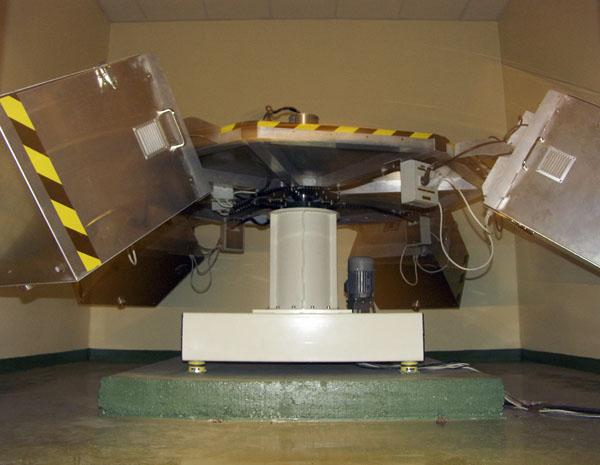
\includegraphics[width=0.7\textwidth]{photo_centrifugeuse.png}
				\caption[Photographie de la centrifugeuse]{Photographie de la centrifugeuse utilisée.}
				\label{photo_centrifugeuse}
			\end{figure}

			\lipsum[2]\index{Nam dui ligula}

\section{Deuxième partie du deuxième chapitre}

	Le faisceau passe ensuite dans un module comprenant un cristal non linéaire permettant de doubler le féquence (excitation de \SIrange{345}{500}{\nano\meter}). Toutes les mesures ont été faites entre \SIlist{400;1200}{\nano\meter} avec un pas de \SI{5}{\nano\meter}.
	
	\lipsum[3]\index{Nulla malesuada}

	\subsection{Première sous-partie de la deuxième partie}

		\lipsum[4]\index{Quisque ullamcorper}

	\subsection[Sous-partie 2]{Deuxième sous-partie de la deuxième partie} % entre [] pour le texte dans la TOC

		Ajout d'une nouvelle entrée d'index de la centrifugeuse\index{centrifugeuse}. Les entrées \gls{+a} \gls{2a} \gls{ca} \gls{Aa} \gls{aa} \gls{alpha} {\NoAutoSpaceBeforeFDP}sont dans la nomenclature. On peux utiliser les commandes personnelles pour appeler rapidement des formules lors de la rédaction \acc et passer des arguments aux commandes pour en modifier l'éxécution \emiss[\nu]{\Omega}.
		
		\subsubsection{Ce titre de partie ne s'affiche pas dans la TOC (tocdepth=2) mais dans la TOC locale (etocsettocdepth=3)}

			Voir (Tableaux~\ref{table:alpha}~et~\ref{table:butcher}).

			\paragraph{Ce titre de partie n'est pas numéroté (secnumdepth=3)}~~\\ % ~~\\ fait le saut de ligne après le titre de 'paragraph' sinon le texte suivant est accolé au titre

				% ce saut de ligne indente le texte de 'paragraph' sinon le paragraphe débute à la marge
				Ajout d'une citation entre parenthèses et tous les auteurs~\parencite{zohdy_mapping_2012}.

			\paragraph{Plusieurs figures côte à côte}~~\\

				\lipsum[66]


				\begin{figure}
					\centering
					\subfloat[Figure A]{\includegraphics[width=.5\textwidth, max height=2in]{example-image-a}}
					\subfloat[Figure B]{\includegraphics[width=.5\textwidth, max height=2in]{example-image-b}}
					\caption{Deux figures}
					\label{fig:deux_figures}
				\end{figure}

			\paragraph{Paramétrer siunitx avec sisetup}~~\\
			
        		Célérité de la lumière dans le vide: $$c=\SI{2.99792458e8}{\meter\per\second}$$
